\documentclass{article}

\usepackage{listings}
\usepackage{enumitem}
\usepackage{amsmath}
\usepackage{mathpazo}
\usepackage{svg}
\usepackage{hyperref}
\hypersetup{
    colorlinks=true,
    linkcolor=blue,
    filecolor=magenta,      
    urlcolor=cyan,
    pdftitle={Overleaf Example},
    pdfpagemode=FullScreen,
    }

\title{CA Lab: Homework 5}
\author{student: Dimitri Tabatadze}

\newcommand{\points}[1]{{\footnotesize{\color{red}\textit{#1 points}}}}

\definecolor{codegreen}{rgb}{0,0.6,0}
\definecolor{codegray}{rgb}{0.5,0.5,0.5}
\definecolor{codepurple}{rgb}{0.58,0,0.82}
\definecolor{backcolour}{rgb}{0.98,0.96,0.94}

\lstdefinestyle{mystyle}{
    backgroundcolor=\color{backcolour},   
    commentstyle=\color{codegreen},
    keywordstyle=\color{magenta},
    numberstyle=\tiny\color{codegray},
    stringstyle=\color{codepurple},
    basicstyle=\ttfamily\footnotesize,
    breakatwhitespace=false,         
    breaklines=true,                 
    captionpos=b,                    
    keepspaces=true,                 
    numbers=left,                    
    numbersep=5pt,                  
    showspaces=false,                
    showstringspaces=false,
    showtabs=false,                  
    tabsize=2
}

\lstset{style=mystyle}

\begin{document}
    \maketitle

    \begin{displaymath}
        \mathbb{N}
    \end{displaymath}

    \section*{Task Description} 
    
    Create the model of a 3-bit register with the signals: reset, set and load. Develop a testbench and simulate the design.

    \begin{enumerate}
        \item Draw the circuits of 3-bit register \points{10}
        \item Create next state table for 3-bit register \points{10}
        \item Write the equations for the next states \points{10}
        \item Write the code of 3-bit register in Verilog \points{60}
    \end{enumerate}

    Please, solve the problems (write the comments) \points{5}, take the clear screenshots and combine all your solutions in one pdf file, then upload in teams. \points{5}

    \section*{Discussion}

    The task is to build a 3 bit parallel register which has 6 inputs:
    \begin{itemize}\setlength\itemsep{0pt}
        \item 3 data,
        \item 1 set,
        \item 1 reset,
        \item 1 load
    \end{itemize}
    bits.
    \begin{enumerate}
        \item when the \verb|reset| bit goes high, all bits of the register should be set to \verb|0|.
        \item whne the \verb|set| bit goes high, all the bits of the register should be set to \verb|1|.
        \item when the \verb|load| bit goes high, the bits of the register should be set to the respective bits of the \verb|data| input.
        \item if none of the above are set, the bits of the register should remain unchanged.
    \end{enumerate}

    \section*{Solution}

    \begin{enumerate}
        \item {
            Here is the circuit diagram:

            \begin{figure}[h]
                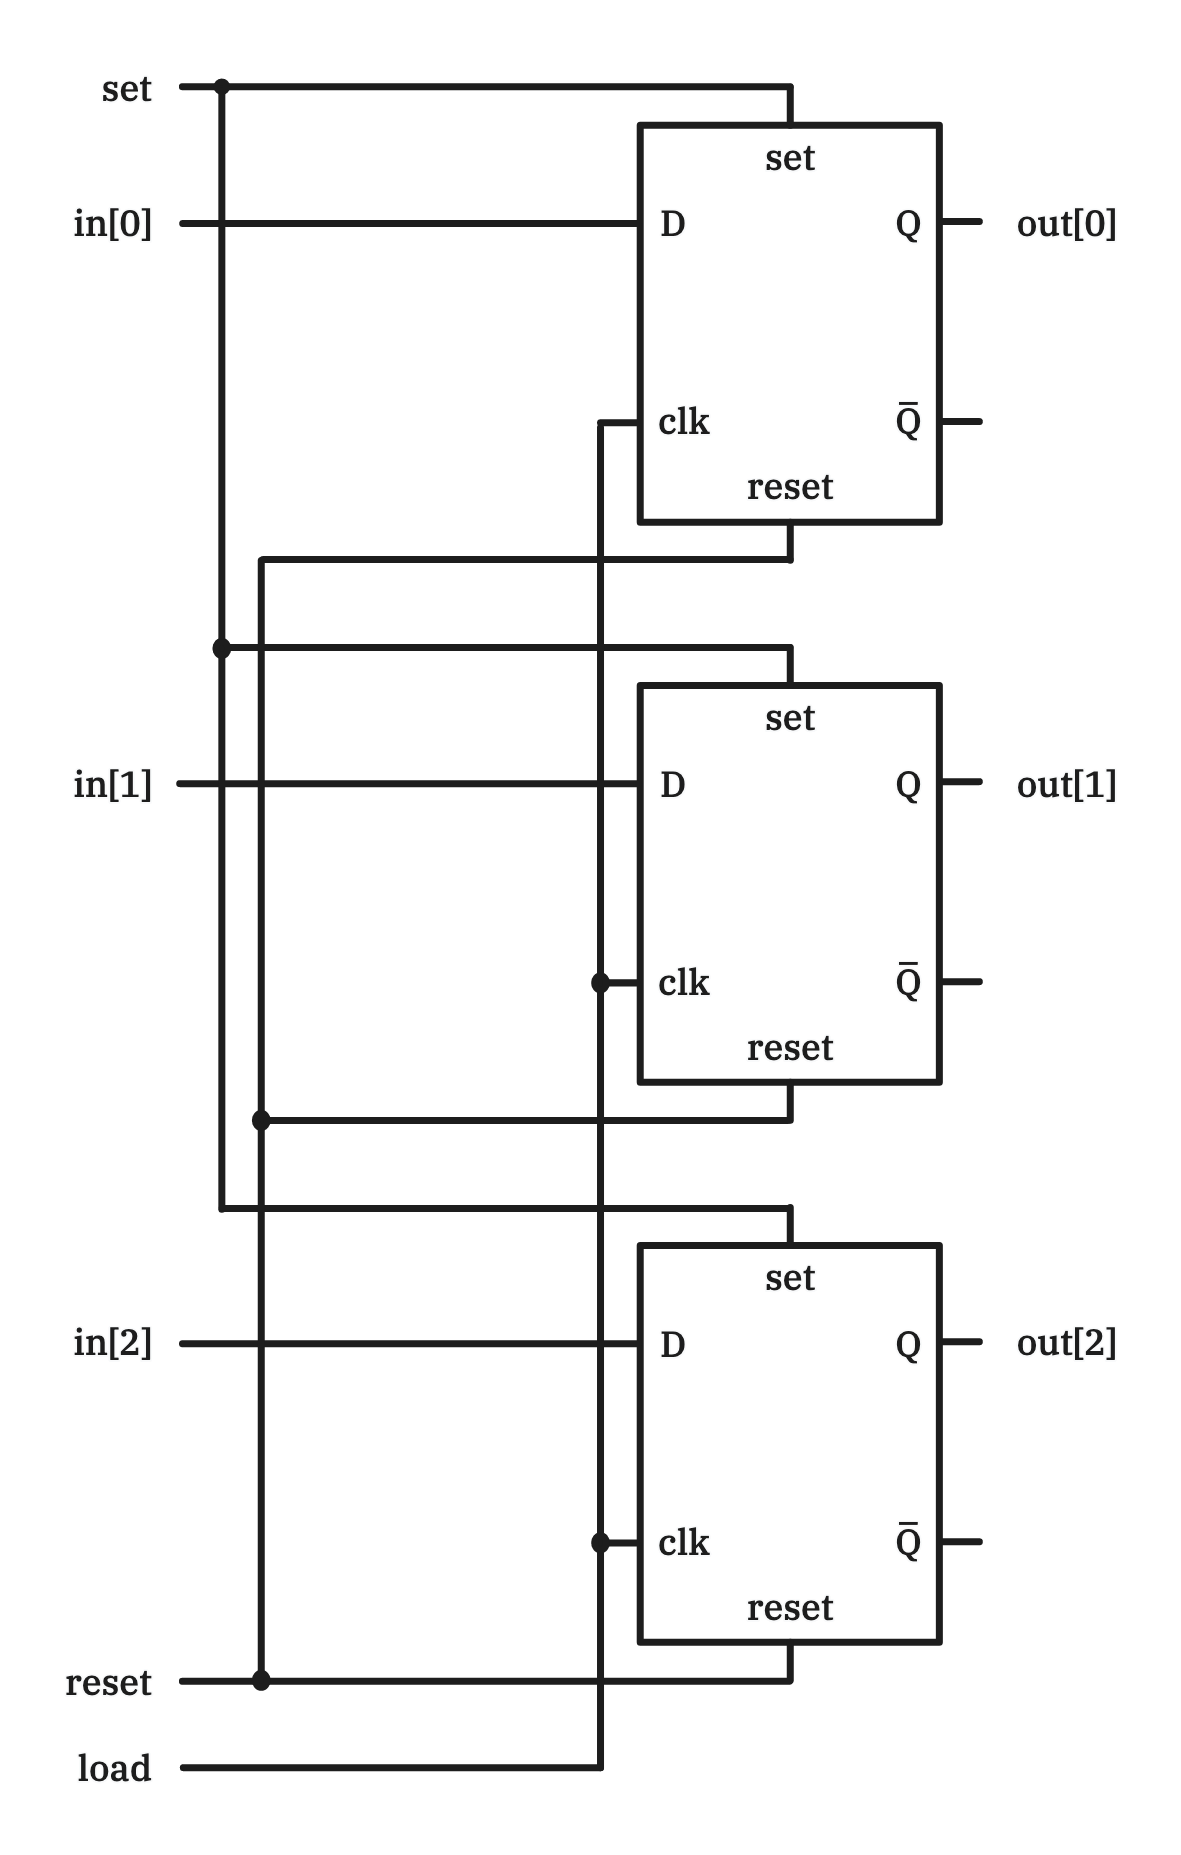
\includegraphics[width=6cm]{diagram.png}
            \end{figure}
        }
        \item {
            \begin{displaymath}
                \begin{array}{| c | c | c | c | c | c | c |}
                    \hline
                    \text{set} & \text{reset} & \text{load} & \text{data} & \text{out} & \text{out}^+ \\
                    \hline \hline
                    0 & 0 & 1 & \texttt{xxx} & \texttt{yyy} & \texttt{xxx} \\ 
                    0 & 1 & 0 & \texttt{xxx} & \texttt{yyy} & 000 \\
                    1 & 0 & 0 & \texttt{xxx} & \texttt{yyy} & 111 \\
                    \hline
                \end{array}
            \end{displaymath}
        }
        \item {
            When the \verb|set| signal goes high:
            \begin{displaymath}
                \begin{aligned}
                    \text{out}^+[0] &= 1 \\
                    \text{out}^+[1] &= 1 \\
                    \text{out}^+[2] &= 1
                \end{aligned}
            \end{displaymath}

            When the \verb|reset| signal goes high:
            \begin{displaymath}
                \begin{aligned}
                    \text{out}^+[0] &= 0 \\
                    \text{out}^+[1] &= 0 \\
                    \text{out}^+[2] &= 0
                \end{aligned}
            \end{displaymath}

            When the \verb|load| signal goes high:
            \begin{displaymath}
                \begin{aligned}
                    \text{out}^+[0] &= in[0] \\
                    \text{out}^+[1] &= in[1] \\
                    \text{out}^+[2] &= in[2]
                \end{aligned}
            \end{displaymath}

            When any of the signals goes low:
            \begin{displaymath}
                \begin{aligned}
                    \text{out}^+[0] &= out[0] \\
                    \text{out}^+[1] &= out[1] \\
                    \text{out}^+[2] &= out[2]
                \end{aligned}
            \end{displaymath}
        }
        \item {
            The Verilog code for a register described above:
            
            \begin{lstlisting}[language=verilog]
module register (
    input reset,
    input load,
    input set,
    input [2:0] data,
    output reg [2:0] out = 0
);

always @(posedge load) begin
    out = data;
end

always @(posedge set) begin
    out = 3'b111;
end

always @(posedge reset) begin
    out = 3'b000;
end

endmodule\end{lstlisting}
        }
    \end{enumerate}

    \section*{Conclusion}

    Although the given task was not so clear with what should have been done, I did what I interpreted the task as. I very much hope that this is correct.

    \section*{Reference}
    
    \begin{itemize}
        \item me
    \end{itemize}

\end{document}